This is a survey of the landscape of 3D visualization in Jupyter Notebooks
performed in March 2017 by Vidar Tonaas Fauske,
to guide \ODK contributions to 3D visualization tools.

\subsection{Summary}

Several packages currently exist that can generate 3D visualizations in
Jupyter Notebooks. This review is intended to give a quick overview of
the current landscape (March 2017), and consider where the contributions
of OpenDreamKit (ODK) can best be directed in order to help improve the
user experience in terms of both features and ease-of-use. The packages
and technologies that will be considered are:

\begin{itemize}
\tightlist
\item
  \href{http://docs.enthought.com/mayavi/mayavi/tips.html\#using-mayavi-in-jupyter-notebooks}{mayavi}
\item
  \href{https://github.com/maartenbreddels/ipyvolume}{ipyvolume}
\item
  \href{http://vispy.org}{vispy}
\item
  \href{https://www.logilab.org/blogentry/8541176}{scivijs}
\item
  \href{https://github.com/K3D-tools/K3D-jupyter}{K3D-jupyter}
\item
  \href{http://vpython.org}{vpython}
\item
  \href{http://nbviewer.jupyter.org/github/sagemanifolds/SageManifolds/blob/master/Worksheets/v1.0/SM_sphere_S2.ipynb}{Sage
  plot3d}
\end{itemize}

Below you can see a (limited) dependency graph between the different
project and technologies. The red text signifies how a kernel package
sends/communicates 3D data to the browser side.

\begin{figure}
\label{fig:pdep}
\centering
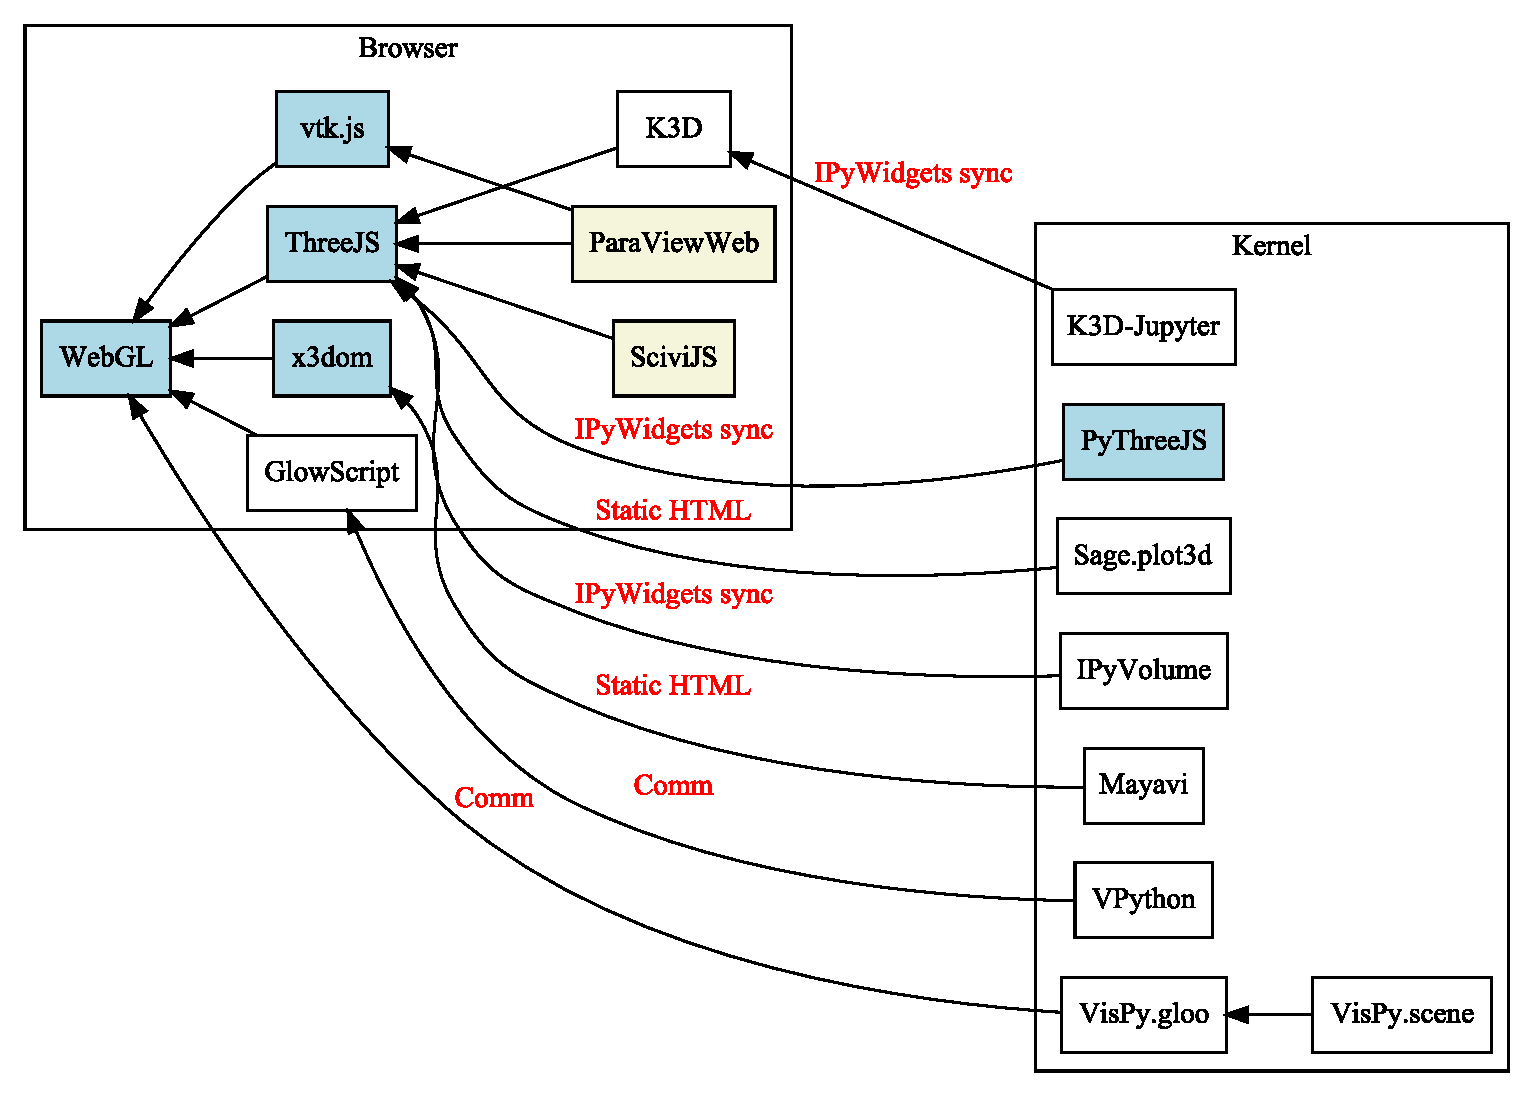
\includegraphics[width=0.6\paperwidth]{existing_tools/dependencies.pdf}
\caption{Package dependency graph}
\end{figure}

As can be seen, there is a variation in how the different projects
couples to WebGL.

\subsubsection{Observations}

Among the packages certain patterns are repeating: - Mayavi and Sage's
plot3d both generate a blob of HTML with x3dom/ThreeJS definitions of
the model + interaction code. This is added as an output of the cell,
and it makes the visualization persistable (i.e.~the view will work the
same with or without a kernel), but it also limits interactivity. -
VPython and VisPy both use temporary displays that are controlled over
Comm. They currently require a roundtrip to the kernel for every frame
draw and/or user interaction. IPyVolume and K3D also uses a temporary
display, but avoids kernel roundtrips by using pre-defined ThreeJS view
controllers. All four packages should be able to persist the views,
e.g.~by recording the executed DOM + Javascript to the output. - Many of
the packages only supply basic inspection tools (a simple camera to
rotate/move). More advanced interactive inspection tools (varying
opacity of different parts, adding and adjusting clipping planes,
tresholding, etc.) are more rare, but could add many benefits to the
user. A possibility here would for ODK to help produce reusable
inspection tools for other visualization tools to use.

In terms of persistence, there are a few things to take into account: -
If the notebook is not trusted, JavaScript is not available, so a static
image should preferrably be saved with the notebook. - Persisting as
HTML with JavaScript is maybe the easiest as it will work out of the box
without any extensions. - Persisting e.g.~x3dom as a separate MIME-type
could enable 3D to work while untrusted (any avenues for code injection
would of course need sanitizing). Would require adding a rendrer through
an nbextension or on the Jupyter level. Adding both this MIME type and
the HTML one on a single output would be nice, but it would nearly
double the output size, which can be significant for larger
geometries/textures.

\subsection{Enabling technology}

\subsubsection{Browser side}

\paragraph{WebGL}

The base layer in terms of enabling technology. All other packages
discussed in this report rely on this.

\paragraph{ThreeJS}

A Javascript framework built on top of WebGL. ThreeJS is the most
prominent WebGL framework today.

Combining custom WebGL code with ThreeJS is not straight forward, but
adding custom shaders is reasonably easy, and ThreeJS should be a
sufficient base for most scientific visualization needs.

\paragraph{x3dom}

A Javascript/XML framework built on top of WebGL. It takes XML as
source, and translates this into a 3D scene. While it sports a
reasonably full feature set, it has not received the same amount of
developer hours as ThreeJS, which can sometimes show. An example of a
simple feature that is missing is an orbit view controller (a ``camera''
orbiting a point, where the up axis is fixed).

\paragraph{vtk.js}

Aims to be (a subset of) VTK built on WebGL. Official project by
Kitware, which plan to transition ParaViewWeb from ThreeJS to it over
time.

\subsubsection{Kernel side (Python)}

\paragraph{PyThreeJS}

A Python bridge to ThreeJS by syncing IPyWidgets.

\begin{quote}
\emph{``This is meant to be a low-level wrapper around three.js. We hope
that others will use this foundation to build higher-level interfaces to
build 3d plots.''}
\end{quote}

\subsection{Higher level interfaces}

\subsubsection{Mayavi}

Mayavi is a high-level interface on top of VTK. It uses x3dom to handle
3D in browser, but also supports a \texttt{png} backend.

Mayavi produces a static HTML output with an x3dom scene generated by
VTK's X3DExporter. VTK also has a WebGLExporter, which is currently not
used by Mayavi.

\paragraph{Installation}

Depends on VTK (\textgreater{}= 5.0) with Python wrappers installed. Not
straight forward to get on all Windows distrubutions, but works nicely
with conda.

The docs says to enable x3dom by installing Mayavi as a notebook
extension, but this has errors. It also bundles an outdated version of
x3dom (bugs out on high-DPI monitor). Simply not installing the Mayavi
nbextension will load the x3dom javascript dynamically from x3dom.org,
which works fine.

\paragraph{Strengths and weaknesses}

Strengths: - Mature package for generating 3D visualization. - Relies on
exporting capabilities of underlying VTK, meaning it should be
reasonably robust. - Output persisted naturally.

Weaknesses: - Requires full re-plot for any changes to the VTK scene;
limited chances for interactivity via e.g.~IPyWidgets. - Requires VTK
installation.

\paragraph{License}

BSD 3-clause

\paragraph{Possible contributions}

\begin{itemize}
\tightlist
\item
  Make a separate notebook/jupyterlab renderer for x3dom MIME type?
\item
  Also add a static PNG snapshot to output MIME bundle.
\end{itemize}

\subsubsection{IPyVolume}

Higher-level package for quickly creating interactive 3D plots of volume
and scatter data. Started December 2016, so still very new.

\paragraph{Installation}

Simple pip install. Package is pure Python + npm package for notebook
extension. Dependencies like Pillow are not pure Python.

Also available on conda.

\paragraph{Strengths and weaknesses}

Strengths: - Integrates well into existing Jupyter environment by
building on top of IPyWidgets. - Good interactivity. - Support for
animations (although limited) with interpolation between frames.

Weaknesses: - Limited capabilities (no lines / surface plotting, no
exploration with e.g.~clip planes, etc.). - Features still need ironing
out / polishing to mature.

\paragraph{License}

MIT

\paragraph{Possible contributions}

\begin{itemize}
\tightlist
\item
  Help mature existing plotting tools.
\item
  Add other high-level functionality like 3D lines / surfaces? That
  might be outside the scope of the package, but a package that does
  something like this might benefit from the communication framework.
\item
  Add interactive exploration controls (clip planes etc.) based on
  IPyWidgets.
\end{itemize}

\subsubsection{K3D}

Described as a \emph{``3D visualization library''}. The specifics of K3D
was not readily apparent, as its documentation is rather thin. However,
the following can be gleamed from the code/examples:

\begin{itemize}
\tightlist
\item
  K3D is intended as a Javascript library for scientific plotting
  (high-level API).
\item
  It uses ThreeJS as a backend (currently the only backend).
\item
  K3D-Jupyter is meant to shim the K3D interface to Jupyter using an
  nbextension (and implements an IPython client using IPyWidgets).
\end{itemize}

K3D might be overlapping in purpose with vtk.js.

\paragraph{Installation}

No release on PyPI/conda yet. Was able to install it from repository
after mucking around with it manually.

\paragraph{Strengths and weaknesses}

Strengths: - Integrates well into existing Jupyter environment by
building on top of IPyWidgets. - Repository control is within control of
ODK participant(s), potentially avoiding conflicts of interest with
other package maintainers.

Weaknesses: - Still immature project. - Installation and documentation
needs work.

\paragraph{License}

MIT

\paragraph{Possible contributions}

\begin{itemize}
\tightlist
\item
  Bring installation/distribution in line with ``Jupyter standard''.
\item
  Ensure optimal use of Jupyter protocol for data transfer across
  kernel/browser interface.
\item
  Documentation.
\item
  Help mature package.
\end{itemize}

\subsubsection{VisPy}

VisPy.app / VisPy.gloo: gloo is a python -\textgreater{} GL abstraction
layer, that supports talking to a WebGL context.

VisPy.scene: High-level visualization interface built on top of gloo.
Still in development, possibly abandoned.

\paragraph{Installation}

\paragraph{Strengths and weaknesses}

Strengths: - Somewhat low-level GL/WebGL access from Python via GLIR
(low-level abstraction on top of various versions of GL/shader
language). - Same interface whether you want to use local GL (in e.g.~a
Qt window) or WebGL in Notebook.

Weaknesses: - Yet another interface wrapper for GL. - User interaction
and timer loops always has to round-trip to kernel side from browser. -
Development seems to has stagnated:

\begin{figure}
\centering
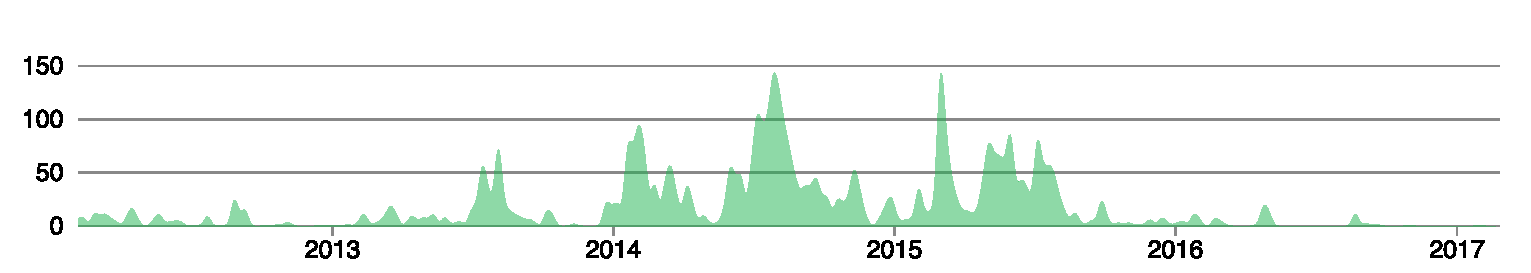
\includegraphics[width=0.6\paperwidth]{existing_tools/vispy_activity.pdf}
\caption{VisPy activity graph}
\end{figure}

\paragraph{License}

BSD 3-Clause

\paragraph{Possible contributions}

\begin{itemize}
\tightlist
\item
  Take over development of high-level part.
\item
  Add view controllers and inspectors to avoid round-trips to kernel
  when in browser.
\item
  Make persisting outputs.
\end{itemize}

\subsubsection{SciviJS}

A node based framework for inspecting/deforming/shading ThreeJS based
geometry. Might overlap in purpose with
\href{https://kitware.github.io/paraviewweb/}{ParaViewWeb}.

\paragraph{Installation}

Installation via \texttt{npm}: unproblematic.

\paragraph{Strengths and weaknesses}

Strengths: - Inspection/exploration tools. - Based on ThreeJS.

Weaknesses: - Still undocumented.

\paragraph{License}

\href{https://opensource.org/licenses/ISC}{ISC}

\paragraph{Possible contributions}

\begin{itemize}
\tightlist
\item
  Enable SciViJS as an inspector for other packages using (Py)ThreeJS
\item
  Help mature the code and add features as needed.
\end{itemize}

\subsubsection{VPython}

Uses GlowScript (sister project) on the browser side to render GL, and
VPython on the kernel side to generate scenes. Implements most things
itself, which means everything is tailored for its purpose, but it loses
out on the benefits of larger libraries. Code can be a bit hard to
follow.

\paragraph{Installation}

Easy install (pip install vpython worked well). A little hard to figure
out which repository/package is the latest. I think this repository is
the main one: https://github.com/BruceSherwood/vpython-jupyter, and
\texttt{vpython} the PyPI package to install. Glowscript is bundled in a
minified version in VPython repository.

\paragraph{Strengths and weaknesses}

Strengths: - Few dependencies. - Active development.

Weaknesses: - Uses quite a lot of browser CPU when idle. - Difficult to
understand code base for someone new.

\paragraph{License}

MIT

\paragraph{Possible contributions}

\begin{itemize}
\tightlist
\item
  Clean up documentation / repositories as someone coming from outside
  with fresh eyes.
\item
  Refactor codebase to ease outside contributions?
\item
  Make persisting outputs
\end{itemize}

\subsubsection{Sage.plot3d}

Uses its own code to convert 3D plots to ThreeJS code, which it embeds
into a static HTML output. As such, it is similar to Mayavi, but is
based on ThreeJS instead of x3dom.

\subsubsection{VTK.js - Jupyter?}

An option would be to implement Jupyter/IPython bindings for vtk.js.

\paragraph{Strengths and weaknesses}

Strengths: - vtk.js has backing of big organization and has a mature
API. - Interface should be familiar to those experienced with VTK. -
Should make it easy to put ParaViewWeb on top for
exploration/inspection. - Possibly good integration with Mayavi?

Weaknesses: - Mostly at mercy of Kitware and their attitude towards
vtk.js (e.g.~if they decide to drop it or it is poorly supported). -
Unkown time-horizon.

\subsection{Concluding remarks}

The following features would all be wanted from a 3D visualization
toolkit for use in Jupyter:

\begin{itemize}
\tightlist
\item
  It should offer a complete API for plotting 3D visualizations.
\item
  More specialized visualizations should hopefully be able to build on
  top of the API for their own purposes.
\item
  It should be open to interactive behavior, while avoiding sending
  redundant information between the kernel and browser.
\item
  It should have tools for inspection/exploration that does not require
  a round-trip to the kernel (syncing inspection parameters is ok, but
  this should not block).
\item
  It would be beneficial if the API could also be used to generate plots
  outside of the Notebook enviornment as well, or at least be able to
  switch to such a tool with little effort.
\item
  The API can benefit greatly by being similar to existing patterns
  (e.g.~Matplotlib or Mayavi/VTK), to ease the learning-curve for new
  users.
\end{itemize}

It is not necessarily aparent which package or combination of packages
are the best to achieve all of these, but the following are examples of
possible solutions: 0. IPyVolume + SciviJS. Uncertain difficulty of
SciviJS integration. 0. K3D + SciviJS 0. ``Jupyter-VTK'': Jupyter
bindings to VTK.js + ParaWebView. Might include Mayavi.
